% ŠABLONA PRO PSANÍ ZÁVĚREČNÉ STUDIJNÍ PRÁCE
%%%%%%%%%%%%%%%%%%%%%%%%%%%%%%%%%%%%%%%%%%%%
% Autor: Jakub Dokulil (kubadokulil99@gmail.com)
% Tato šablona byla vytvořena tak, aby pomocí ní mohli v systému LaTeX soutěžící sázet své práce a zároveň odpovídala požadavkům na formátování vyplývajícím z wordové šablony umístěné na webu soc.cz.
%
\documentclass[12pt, a4paper,
%oneside,      %% -- odkomentujte, pokud chcete svou práci mít pouze jednostrannou, mezera pro hřbet pak automaticky bude pouze na levé straně
twoside,        %% -- pro oboustranné práce, mezera pro hřbet následně střídá strany.
openright
]{report}

%% Nutné balíčky a nastavení
%%%%%%%%%%%%%%%%%%%%%%%%%%%%

%% Proměnné
\newcommand\obor{INFORMAČNÍ TECHNOLOGIE} %% -- napiš číslo a název tvého oboru
\newcommand\kodOboru{18-20-M/01} %% -- napiš číslo a název tvého oboru
\newcommand\zamereni{se zaměřením na počítačové sítě a programování} %% -- napiš číslo a název tvého oboru
\newcommand\skola{Střední škola průmyslová a umělecká, Opava} %% vyplň název školy
\newcommand\trida{IT4} %% vyplň jméno svého konzultanta
\newcommand\jmenoAutora{Viktor Hujer}  %% vyplň své jméno
\newcommand\skolniRok{2023/24} %% vyplň rok
\newcommand\datumOdevzdani{1. 1. 2024} %% vyplň rok
\newcommand\nazevPrace{Tvorba odborné dokumentace s využitím typografického systému \LaTeX} %% vyplň název své práce

\title{\nazevPrace} %% -- Název tvé práce
\author{\jmenoAutora} %% -- tvé jméno
\date{\datumOdevzdani} %% -- rok, kdy píšeš SOČku

\usepackage[top=2.5cm, bottom=2.5cm, left=3.5cm, right=1.5cm]{geometry} %% nastaví okraje, left -- vnitřní okraj, right -- vnější okraj

\usepackage[czech]{babel} %% balík babel pro sazbu v češtině
\usepackage[utf8]{inputenc} %% balíky pro kódování textu
\usepackage[T1]{fontenc}
\usepackage{cmap} %% balíček zajišťující, že vytvořené PDF bude prohledávatelné a kopírovatelné

\usepackage{graphicx} %% balík pro vkládání obrázků

\usepackage{subcaption} %% balíček pro vkládání podobrázků

\usepackage{hyperref} %% balíček, který v PDF vytváří odkazy

\linespread{1.25} %% řádkování
\setlength{\parskip}{0.5em} %% odsazení mezi odstavci


\usepackage[pagestyles]{titlesec} %% balíček pro úpravu stylu kapitol a sekcí
\titleformat{\chapter}[block]{\scshape\bfseries\LARGE}{\thechapter}{10pt}{\vspace{0pt}}[\vspace{-22pt}]
\titleformat{\section}[block]{\scshape\bfseries\Large}{\thesection}{10pt}{\vspace{0pt}}
\titleformat{\subsection}[block]{\bfseries\large}{\thesubsection}{10pt}{\vspace{0pt}}


\usepackage{tocloft} % Balíček umožní přizpůsobit vzhled tabulky obsahu
\setlength{\cftbeforechapskip}{0pt}  % Menší rozestup pro kapitoly
\setlength{\cftbeforesecskip}{0pt}   % Menší rozestup pro sekce

\setcounter{secnumdepth}{2}
\setcounter{tocdepth}{1}
\usepackage{fancyhdr}
\pagestyle{fancy}
\renewcommand{\headrulewidth}{0.025pt}

\usepackage{booktabs}

\usepackage{url}

%% Balíčky co se můžou hodit :) 
%%%%%%%%%%%%%%%%%%%%%%%%%%%%%%%

\usepackage{pdfpages} %% Balíček umožňující vkládat stránky z PDF souborů, 

\usepackage{upgreek} %% Balíček pro sazbu stojatých řeckých písmen, třeba u jednotky mikrometr. Například stojaté mí: \upmu, stojaté pí: \uppi

\usepackage{amsmath}    %% Balíčky amsmath a amsfonts 
\usepackage{amsfonts}   %% pro sazbu matematických symbolů
\usepackage{esint}     %% pro sazbu různých integrálů (např \oiint)
\usepackage{mathrsfs}
\usepackage{helvet} % Helvet font
\usepackage{mathptmx} % Times New Roman
\usepackage{Oswald} % Oswald font


%% makra pro sazbu matematiky
\newcommand{\dif}{\mathrm{d}} %% makro pro sazbu diferenciálu, místo toho
%% abych musel psát '\mathrm{d}' mi stačí napsat '\dif' což je mnohem 
%% kratší a mohu si tak usnadnit práci

\usepackage{listings}
\usepackage{xcolor}

\renewcommand{\lstlistingname}{Kód}% Listing -> Algorithm
\renewcommand{\lstlistlistingname}{Seznam programových kódů}% List of Listings -> List of Algorithms

%% Definice 
\lstdefinelanguage{JavaScript}{
	morekeywords=[1]{break, continue, delete, else, for, function, if, in,
		new, return, this, typeof, var, void, while, with},
	% Literals, primitive types, and reference types.
	morekeywords=[2]{false, null, true, boolean, number, undefined,
		Array, Boolean, Date, Math, Number, String, Object},
	% Built-ins.
	morekeywords=[3]{eval, parseInt, parseFloat, escape, unescape},
	sensitive,
	morecomment=[s]{/*}{*/},
	morecomment=[l]//,
	morecomment=[s]{/**}{*/}, % JavaDoc style comments
	morestring=[b]',
	morestring=[b]"
}[keywords, comments, strings]


\lstdefinelanguage[ECMAScript2015]{JavaScript}[]{JavaScript}{
	morekeywords=[1]{await, async, case, catch, class, const, default, do,
		enum, export, extends, finally, from, implements, import, instanceof,
		let, static, super, switch, throw, try},
	morestring=[b]` % Interpolation strings.
}

\lstalias[]{ES6}[ECMAScript2015]{JavaScript}

% Nastavení barev
% Requires package: color.
\definecolor{mediumgray}{rgb}{0.3, 0.4, 0.4}
\definecolor{mediumblue}{rgb}{0.0, 0.0, 0.8}
\definecolor{forestgreen}{rgb}{0.13, 0.55, 0.13}
\definecolor{darkviolet}{rgb}{0.58, 0.0, 0.83}
\definecolor{royalblue}{rgb}{0.25, 0.41, 0.88}
\definecolor{crimson}{rgb}{0.86, 0.8, 0.24}

% Nastavení pro Python
\lstdefinestyle{Python}{
	language=Python,
	backgroundcolor=\color{white},
	basicstyle=\ttfamily,
	breakatwhitespace=false,
	breaklines=false,
	captionpos=b,
	columns=fullflexible,
	commentstyle=\color{mediumgray}\upshape,
	emph={},
	emphstyle=\color{crimson},
	extendedchars=true,  % requires inputenc
	fontadjust=true,
	frame=single,
	identifierstyle=\color{black},
	keepspaces=true,
	keywordstyle=\color{mediumblue},
	keywordstyle={[2]\color{darkviolet}},
	keywordstyle={[3]\color{royalblue}},
	literate=%
	{á}{{\'a}}1 {č}{{\v{c}}}1 {ď}{{\v{d}}}1 {é}{{\'e}}1 {ě}{{\v{e}}}1
	{í}{{\'i}}1 {ň}{{\v{n}}}1 {ó}{{\'o}}1 {ř}{{\v{r}}}1 {š}{{\v{s}}}1
	{ť}{{\v{t}}}1 {ú}{{\'u}}1 {ů}{{\r{u}}}1 {ý}{{\'y}}1 {ž}{{\v{z}}}1,		
	numbers=left,
	numbersep=5pt,
	numberstyle=\tiny\color{black},
	rulecolor=\color{black},
	showlines=true,
	showspaces=false,
	showstringspaces=false,
	showtabs=false,
	stringstyle=\color{forestgreen},
	tabsize=2,
	title=\lstname,
	upquote=true  % requires textcomp	
}


\lstdefinestyle{JSES6Base}{
	backgroundcolor=\color{white},
	basicstyle=\ttfamily,
	breakatwhitespace=false,
	breaklines=false,
	captionpos=b,
	columns=fullflexible,
	commentstyle=\color{mediumgray}\upshape,
	emph={},
	emphstyle=\color{crimson},
	extendedchars=true,  % requires inputenc
	fontadjust=true,
	frame=single,
	identifierstyle=\color{black},
	keepspaces=true,
	keywordstyle=\color{mediumblue},
	keywordstyle={[2]\color{darkviolet}},
	keywordstyle={[3]\color{royalblue}},
 literate=%
{á}{{\'a}}1 {č}{{\v{c}}}1 {ď}{{\v{d}}}1 {é}{{\'e}}1 {ě}{{\v{e}}}1
{í}{{\'i}}1 {ň}{{\v{n}}}1 {ó}{{\'o}}1 {ř}{{\v{r}}}1 {š}{{\v{s}}}1
{ť}{{\v{t}}}1 {ú}{{\'u}}1 {ů}{{\r{u}}}1 {ý}{{\'y}}1 {ž}{{\v{z}}}1,		
	numbers=left,
	numbersep=5pt,
	numberstyle=\tiny\color{black},
	rulecolor=\color{black},
	showlines=true,
	showspaces=false,
	showstringspaces=false,
	showtabs=false,
	stringstyle=\color{forestgreen},
	tabsize=2,
	title=\lstname,
	upquote=true  % requires textcomp
}

\lstdefinestyle{JavaScript}{
	language=JavaScript,
	style=JSES6Base,
}
\lstdefinestyle{ES6}{
	language=ES6,
	style=JSES6Base
}


%% Bordel pro práci - můžeš smáznout :) 
%%%%%%%%%%%%%%%%%%%

\usepackage{lipsum} %% balíček který píše lipsum (nesmyslný text, který se používá pro kontrolu typografie)

%% Začátek dokumentu
%%%%%%%%%%%%%%%%%%%%
\begin{document}
	
	\pagestyle{empty}
	\pagenumbering{Roman}
	
	\cleardoublepage

%% Titulní stránka s informacemi
%%%%%%%%%%%%%%%%%%%%%%%%%%%%%%%%%%%%%%%%
	
	{\fontfamily{phv}\selectfont
		%% Logo školy
		\begin{figure}[h]
			\centering
			
\includegraphics[width=0.6\linewidth]{image/logo-skoly.png} 
		\end{figure}
		
		
		%% Hlavička práce a její název (viz proměnná \nazev prace)
		%% \sffamily %%% bezpatkové písmo - sans serif
		{\bfseries %%% písmo na stránce je tučně
			\begin{center}
				\vspace{0.025 \textheight}
				\LARGE{ZÁVĚREČNÁ STUDIJNÍ PRÁCE}\\
				\large{dokumentace}\\
				\vspace{0.075 \textheight}
				\LARGE {\nazevPrace}\\
			\end{center}  
		}%%%
		
		\begin{figure}[h]
			\centering
			
\includegraphics[width=0.8\linewidth]{image/programovani-02.jpg} 
		\end{figure}
		
		\vspace{0.02 \textheight}
		\begin{table}[h!]
			\begin{tabular}{ll}
				\textbf{Autor:} & \jmenoAutora\\ 
				\textbf{Obor:} & \kodOboru { } \obor\\
				\textbf{} & \zamereni\\
				\textbf{Třída:} & \trida\\
				\textbf{Školní rok:} & \skolniRok\\
			\end{tabular}
			
		\end{table}		
	}
	
\cleardoublepage %% Zalomení dvojstránky
	
%% Stránka obsahující poděkování a prohlášení
%%%%%%%%%%%%%%%%%%%%%%%%%%%%%%%%%%%%%%%%%%%%%%%%%%%%%%%%

%% Poděkování - nepovinné
%%%%%%%%%%%%%%%%%%%%%%%%%%%%
	
	\noindent{\large{\bfseries{Poděkování}\\}}
	\noindent Prostor k poděkování (například vedoucímu práce).
	
	\vspace*{0.7\textheight} %% Vertikální mezeru je možné upravit

%% Prohlášení - povinné
%%%%%%%%%%%%%%%%%%%%%%%%%%%%
	\noindent{\large{\bfseries{Prohlášení}\\}}  %% uprav si koncovky podle toho na jaký rod se cítíš, vypadá to pak lépe :) 
	\noindent{Prohlašuji, že jsem závěrečnou práci vypracoval samostatně a uvedl veškeré použité 
		informační zdroje.\\}
	\noindent{Souhlasím, aby tato studijní práce byla použita k výukovým a prezentačním účelům na Střední průmyslové a umělecké škole v Opavě, Praskova 399/8.}
	\vfill
	\noindent{V Opavě \datumOdevzdani\\}
	\noindent
	\begin{minipage}{\linewidth}
		\hspace{9.5cm} 
		\begin{tabular}{@{}p{6cm}@{}}
			\dotfill \\
			Podpis autora
		\end{tabular}
	\end{minipage}
	
	\cleardoublepage %% Zalomení dvojstránky

%% Stránka obsahující abstrakt (anotaci)
%%%%%%%%%%%%%%%%%%%%%%%%%%%%%%%%%%%%%%%%%%%%%%%%%%%%%%%%	

%% Abstrakt v češtině
%%%%%%%%%%%%%%%%%%%%%%%%%%%%
	\noindent{\Large{\bfseries{Abstrakt}\\}}
	\noindent Sem napíšeš svůj abstrakt.\\
	Slouží jako pomoc čtenáři rychle se zorientovat v dané práci.\\
	“Redukovaný text, který charakterizuje obsah dokumentu bez rozlišování autorství abstraktu, bez doplňkových informací, bez vlastní interpretace a hodnocení dokumentu (tj. nikoliv "v práci velmi dobře hodnotím podle mne zajímavý systém...", ale "práce hodnotí systém..."). Základními vlastnostmi anotace jsou výstižnost, přehlednost, jasnost, stručnost, přesnost, objektivnost a čtivost. Anotace je formulována v přirozeném jazyce – obvykle ve větách. Anotace může používat textových formulací z referovaného dokumentu, ale jako celek je formulován nově.“\\
	Délka cca 100 – 250 slov
	
	\vspace{18pt}
	
	\noindent{\large{\bfseries{Klíčová slova}}}
	
	\noindent Šablona, \LaTeX, závěrečná práce, dokumentace, \dots 
	
	\vspace{18pt}

%% Abstrakt v angličtině
%%%%%%%%%%%%%%%%%%%%%%%%%%%%	
	\noindent{\Large{\bfseries{Abstract}}}
	
	\noindent Write your abstract here! \lipsum[1] %% přepiš!!
	
	\vspace{18pt}
	
	\noindent{\large{\bfseries{Keywords}}}
	
	\noindent Template, \LaTeX, High school proffessional activity, \dots 
	
	\clearpage %% Zalomení stránky

%% Stránka s generovaným obsahem
%%%%%%%%%%%%%%%%%%%%%%%%%%%%%%%%%%%%%%%	
	
	\tableofcontents %% Vygeneruje tabulku s obsahem

	\pagenumbering{arabic} %% Nastavení způsobu číslování stránek (alternativy roman | Roman)
	\setcounter{page}{1} %% Nastavení počitadla stránek

%% Stránka s úvodem - povinná část
%%%%%%%%%%%%%%%%%%%%%%%%%%%%%%%%%%%%%%%		
	\chapter*{Úvod}
%Tento příkaz vytvoří novou kapitolu s názvem "Úvod" ve vašem dokumentu.
%Hvězdička * u příkazu \chapter* znamená, že tato kapitola nebude mít číslo. Ve výsledném dokumentu se tedy objeví jako "Úvod" bez předcházejícího čísla kapitoly, které se obvykle zobrazuje u číslovaných kapitol.
%Tento příkaz také znamená, že kapitola se automaticky neobjeví v obsahu, protože LaTeX standardně zahrnuje do obsahu pouze číslované kapitoly.
	\addcontentsline{toc}{chapter}{Úvod}
%Tento příkaz ručně přidává záznam do obsahu.
%První parametr toc označuje, že přidáváme záznam do Table of Contents (obsahu).
%Druhý parametr chapter specifikuje úroveň záznamu. V tomto případě říkáme, že přidávaný záznam má být považován za kapitolu.
%Třetí parametr Úvod je text, který se objeví v obsahu. V tomto případě bude v obsahu zobrazen název "Úvod".	
Závěrečné studijní práce a jejich veřejné obhajoby jsou důležitou součástí vyvrcholení studia oboru informační technologie na \textit{Střední škole průmyslové a umělecké v Opavě}. Hlavním cílem je samostatně vypracovat komplexní, nejčastěji prakticky zaměřený projekt na vybrané téma z~oblasti ICT a napsat k tomuto projektu také příslušnou odbornou dokumentaci podle obecně platných pravidel. Nejúspěšnější studentské projekty bývají vybrány, aby školu reprezentovaly v soutěžních přehlídkách \emph{Středoškolské odborné činnosti} (dále SOČ), kde je pečlivá a přesná dokumentace rovněž vyžadována.

Tento dokument vznikl se záměrem co nejvíce studentům usnadnit formální úpravu dokumentace k jejich odborné práci a poskytnout jim i dobré vodítko při strukturování samotného obsahu. Vzhledem k tomu, že příprava na vysokoškolské studium často vyžaduje znalost {\LaTeX}u, představujeme šablonu vytvořenou v této technologii, jejímž autorem je z velké části Jakub Dokulil a která byla původně určená pro soutěžící SOČ.  

První kapitola této práce obsahuje základní informace o~{\LaTeX}u; stručně se zmiňuje o jeho vývoji, ale hlavně se soustředí na základní principy, které je nezbytné znát při sestavování rozsáhlejších  textových dokumentů. Součástí této kapitoly je i výběr některých programových prostředků, které mohou výrazněji urychlit a usnadnit psaní zdrojového kódu {\LaTeX}u. V kapitole nazvané "Jak psát odbornou dokumentaci" jsou zdůrazněna nejdůležitější pravidla, jež by měla být dodržena při psaní (nejen) odborného textu, a to jak zásady týkající se obsahu, tak i formální stránky - pravopisné, typografické apod. Závěrečná kapitola se soustředí na praktické ukázky správného použití různých typů obsahu v odborné práci. 

%Tipy k psaní úvodu
%Je povinný, nadpis neměňte, rozsah - max. 1 strana. 
%Tato část práce obsahuje: 
%* náhled do řešené problematiky, zdůvodnění volby problematiky, 
%* předem definované cíle práce, 
%* motivaci pro další čtení textu včetně stručného uvedení obsahu následujících kapitol 


\chapter{Typografický systém LaTeX}

\section{Úvod}
\label{sec:uvod}

V této kapitole se seznámíme s \LaTeX{}, což je vysoko kvalitní typografický systém, speciálně navržený pro produkci technické a vědecké dokumentace. \LaTeX{} je široce používán akademiky, vědci, inženýry a dalšími profesionály, kteří potřebují efektivně vytvářet vysoce kvalitní dokumenty, jako jsou články, reporty, knihy a dokonce i prezentace.

\subsection{Co je \LaTeX{}}
\LaTeX{} je založen na programu \TeX{}, který byl původně vytvořen Donaldem E. Knuthem v pozdních 70. letech. Na rozdíl od běžných textových procesorů, které jsou "What You See Is What You Get" (WYSIWYG), \LaTeX{} funguje na principu "What You See Is What You Mean" (WYSIWYM). To znamená, že se uživatelé soustředí na strukturu a obsah svého textu, zatímco vzhled dokumentu je řízen předdefinovanými šablonami.

\subsection{Výhody používání \LaTeX{}}
Hlavní výhodou používání \LaTeX{} je jeho schopnost vytvářet profesionálně vypadající dokumenty s konzistentním formátováním. Dále nabízí:

\begin{itemize}
	\item Vynikající kvalitu sazby, zvláště pro matematické vzorce.
	\item Automatizované generování obsahu, seznamů obrázků, tabulek a bibliografických odkazů.
	\item Možnost snadno pracovat s komplexními dokumenty jako jsou disertace nebo knihy.
	\item Rozsáhlé možnosti přizpůsobení a širokou škálu balíčků rozšiřujících jeho funkčnost.
\end{itemize}

V následujících sekcích se podrobněji podíváme na základní prvky \LaTeX{} a naučíme se, jak je používat k vytváření kvalitních dokumentů.


\section{Základní struktura dokumentu}
\label{sec:zakladni_struktura}

V této kapitole se podrobněji podíváme na základní strukturu dokumentu v \LaTeX{}u. Po porozumění této struktuře budete schopni vytvářet vlastní dokumenty s přizpůsobeným formátováním a strukturou.

\subsection{Preambule dokumentu}
Preambule je první částí každého \LaTeX{}ového dokumentu. Zde definujeme typ dokumentu, který chceme vytvořit, a nastavíme různé parametry, které ovlivňují celkový vzhled dokumentu. Preambule také často obsahuje příkazy pro načítání různých balíčků, které rozšiřují základní funkčnost \LaTeX{}u.

\begin{verbatim}
	\documentclass[options]{class}
	\usepackage[options]{package}
\end{verbatim}

\subsection{Hlavní tělo dokumentu}
Hlavní tělo dokumentu začíná příkazem \verb|\begin{document}| a končí \verb|\end{document}|. Veškerý obsah, který chcete mít ve svém dokumentu, by měl být umístěn mezi tyto dva příkazy. 

\subsection{Sekce a podsekce}
Pro organizaci obsahu se často používají sekce a podsekce. Tyto struktury pomáhají čtenáři lépe navigovat dokumentem a rozdělit text do logických bloků.

\begin{verbatim}
	\section{Název sekce}
	\subsection{Název podsekce}
	\subsubsection{Název podpodsekce}
\end{verbatim}

\subsection{Odstavce a rozestupy}
V \LaTeX{}u je nový odstavec vytvořen jednoduše vložením jedné nebo více prázdných řádek. Rozestupy mezi odstavci, stejně jako zarovnání textu, můžeme upravit podle potřeby.

\section{Práce s textem}
\label{sec:prace_s_textem}

Tato část se zaměřuje na základní techniky práce s textem v \LaTeX{}u, včetně formátování textu, vytváření seznamů a využití křížových odkazů a poznámek pod čarou.

\subsection{Formátování textu}
Formátování textu je klíčovým prvkem pro zvýraznění důležitých informací a zlepšení čitelnosti dokumentu.

\subsubsection{Zvýraznění textu}
V \LaTeX{}u existuje několik způsobů, jak zvýraznit text. Můžeme použít tučné písmo, kurzívu nebo podtržení.

\begin{verbatim}
	\textbf{tučné písmo}, \textit{kurzíva}, \underline{podtržený text}
\end{verbatim}

\subsubsection{Seznamy a výčty}
Seznamy jsou užitečné pro strukturování informací a jejich uspořádání do čitelné formy. \LaTeX{} podporuje nečíslované, číslované a popisné seznamy.

\begin{verbatim}
	\begin{itemize}
		\item Nečíslovaný seznam
	\end{itemize}
	
	\begin{enumerate}
		\item Číslovaný seznam
	\end{enumerate}
	
	\begin{description}
		\item[Popisek] Popisný seznam
	\end{description}
\end{verbatim}

\subsection{Křížové odkazy a poznámky pod čarou}
Křížové odkazy a poznámky pod čarou jsou důležité pro odkazování na jiné části dokumentu a poskytování dodatečných informací.

\subsubsection{Křížové odkazy}
Pomocí křížových odkazů můžeme odkazovat na jiné sekce, obrázky nebo tabulky v dokumentu.

\begin{verbatim}
	\label{sec:nazev_sekce}
	Odkaz na sekci \ref{sec:nazev_sekce}.
\end{verbatim}

\subsubsection{Poznámky pod čarou}
Poznámky pod čarou poskytují dodatečné informace bez přerušení toku hlavního textu.

\begin{verbatim}
	Text s poznámkou pod čarou.\footnote{Text poznámky pod čarou.}
\end{verbatim}



\section{Matematické vzorce a symboly}
\label{sec:matematicke_vzorce_a_symboly}

Tato část poskytuje přehled o vkládání matematických vzorců a symbolů do dokumentů v \LaTeX{}u, což je nezbytné pro tvorbu akademických a vědeckých textů.

\subsection{Základní matematické prostředí}
\LaTeX{} nabízí několik prostředí pro práci s matematikou, včetně "math" pro základní matematické výrazy a "displaymath" pro samostatné rovnice.

\begin{verbatim}
	$z = x + y$ % Inline matematika
	\begin{displaymath}
		z = x + y
	\end{displaymath}
\end{verbatim}

\subsection{Rovnice a symboly}
Matematické rovnice a symboly jsou základem mnoha vědeckých dokumentů, a \LaTeX{} poskytuje širokou škálu nástrojů pro jejich efektivní použití.

\subsubsection{Vložení jednoduché rovnice}
Pro vložení jednoduché rovnice můžeme použít prostředí "equation" nebo "align" pro více rovnic s zarovnáním.

\begin{verbatim}
	\begin{equation}
		E = mc^2
	\end{equation}
\end{verbatim}

\subsubsection{Pokročilé matematické výrazy}
Pro složitější matematické výrazy, jako jsou integrály, sumy nebo frakce, \LaTeX{} nabízí rozsáhlé možnosti.

\begin{verbatim}
	\begin{equation}
		\int_0^\infty e^{-x} \, dx
	\end{equation}
\end{verbatim}



\section{Práce s obrázky a tabulkami}
\label{sec:prace_s_obrazky_a_tabulkami}

Tato kapitola je zaměřena na vkládání a formátování obrázků a tabulek v \LaTeX{}u, což jsou klíčové dovednosti pro vytváření vizuálně atraktivních a informativních dokumentů.

\subsection{Vkládání obrázků}
Vkládání obrázků do dokumentů \LaTeX{}u umožňuje autorům přidávat vizuální prvky, které podporují a doplňují textový obsah.

\subsubsection{Formáty obrázků}
\LaTeX{} podporuje různé formáty obrázků, včetně populárních formátů jako JPEG, PNG a PDF. Výběr správného formátu je důležitý pro kvalitu a velikost souboru.

\begin{verbatim}
	\includegraphics[width=0.5\textwidth]{obrazek.jpg}
\end{verbatim}

\subsubsection{Pozicování obrázků}
Správné pozicování obrázků je klíčové pro zachování čitelnosti a estetiky dokumentu. \LaTeX{} nabízí několik možností, jak ovlivnit umístění obrázků v textu.

\begin{verbatim}
	\begin{figure}[h]
		\centering
		\includegraphics[width=0.5\textwidth]{obrazek.jpg}
		\caption{Popisek obrázku}
		\label{fig:obrazek}
	\end{figure}
\end{verbatim}

\subsection{Vytváření tabulek}
Tabulky jsou nezbytné pro organizované a efektivní prezentování dat. \LaTeX{} umožňuje vytváření jak jednoduchých, tak složitých tabulek.

\subsubsection{Základní tabulky}
Pro vytváření základních tabulek lze využít prostředí "tabular". Jednoduchá tabulka může být vytvořena bez složitých formátovacích nástrojů.

\begin{verbatim}
	\begin{tabular}{|c|c|c|}
		\hline
		A & B & C \\
		\hline
		1 & 2 & 3 \\
		\hline
	\end{tabular}
\end{verbatim}

\subsubsection{Pokročilé tabulky}
Pro složitější tabulky, jako jsou tabulky s více řádky nebo sloupci, lze použít pokročilé formátovací možnosti, jako jsou sloučené buňky a speciální zarovnání.

\begin{verbatim}
	\begin{table}[h]
		\centering
		\begin{tabular}{|c|c|c|}
			\hline
			\multirow{2}{*}{A} & B1 & C1 \\
			\cline{2-3}
			& B2 & C2 \\
			\hline
		\end{tabular}
		\caption{Pokročilá tabulka}
		\label{tab:pokrocila_tabulka}
	\end{table}
\end{verbatim}



\section{Bibliografie a citace}
\label{sec:bibliografie_a_citace}

Tato kapitola poskytuje podrobný návod na vytváření bibliografie a správné citování zdrojů v \LaTeX{}u, což jsou nezbytné dovednosti pro akademické psaní a publikování.

\subsection{Vytváření bibliografie}
\LaTeX{} umožňuje efektivní správu bibliografických záznamů a jejich automatické formátování. Tento proces zahrnuje několik kroků od definování zdrojů po jejich začlenění do dokumentu.

\begin{verbatim}
	\begin{thebibliography}{99}
		\bibitem{nazev}
		Autor, \emph{Název knihy}, Nakladatelství, Rok.
	\end{thebibliography}
\end{verbatim}

\subsection{Citování zdrojů}
Správné citování zdrojů je klíčové pro akademickou integritu a umožňuje čtenářům dohledat zmiňované informace. V \LaTeX{}u je možné citovat zdroje jednoduše pomocí příkazu \verb|\cite|.

\begin{verbatim}
	Jak bylo zmíněno v \cite{nazev}, ...
\end{verbatim}



	

	\chapter{Tipy k psaní}
	\pagestyle{fancy}
	Jak už jsem psal výše \LaTeX je dosti komplexní systém, který umožňuje psát velmi rozsáhlé text. Jeho autor Donald Knuth ho stvořil, aby mohl vydat jeho učebnici \emph{The Art of Computer Programming} a dodnes se je využíván pro sazbu skript, učebnic, článků či závěrečných prací. V této kapitole najdeš ukázky různých funkcí a balíčků \LaTeX u od těch nejzákladnějších až po složitější. Neznamená to nutně, že všechny musíš použít, ale když potřebuješ pomoct, tak je dobré mít oporu. 
	
	Pokud s \LaTeX em úplně začínáš tak ti můžu doporučit přiručku \emph{Ne příliš stručný úvod do systému \LaTeX2e}~\cite{LaTeXprirucka}. Případně spoustu užitečných informací nalezneš na Wikibooks~\cite{wikibooksLaTeX}. Pokud narazíš na nějaký problém googli. Na internetu je spoustu fór, kde pravděpodobně už někdo podobný problém řešil. Asi nejvíce otho najdeš na stránce \emph{TeX - LaTeX Stackexchange} \cite{stackExchange}.
	
	
	\section[Základy]{Základy: Text, obrázky, tabulky a citace} %%[Text, který bude v obsahu]{Text, který se vytiskne na stránce} Zkus měnit jednotlivé závorky a uvidíš :) 
	Psaní v \LaTeX{u} není žádná věda, stačí psát normálně do zdrojového souboru. Pokud bys chtěl psát obrážky či číslovaný seznam, pak můžeš použít prostředí \texttt{itemize} či \texttt{enumerate}. Často je důležité používat nezlomitelnou mezeru. Tu uděláš pomocí \verb|~|~(tildy). Pokud budeš chtít psát uvozovky použij příkaz \texttt{uv}, pomocí něj se ti vytvoří uvozovky podle příslušného jazyka. V česku tedy ve formátu 99 66. Použití příkazu najdeš níže v textu.
	
	Občas je zapotřebí \LaTeX{u} pomoct při rozdělování slov. To se udělá snadno vložením symbolů \verb|\-| mezi jednotlivé slabiky.
	
	\subsection{Tabulky}
	
	U tabulek platí to stejné co u obrázků. Zarovnávají se na střed a nechávají se \uv{plavat} v textu. Tabulka narozdíl od textu, má popisek nahoře. U tabulky \ref{tab:ukazka} je použit balíček \texttt{booktabs}, pomocí kterého je celá tabulka naformátovaná.
	
	Seznam jak obrázků tak tabulek je pak vytvořen pomocí příkazů \texttt{listoftables} a~\texttt{list\-of\-fig\-ures} na konci práce před literaturou.
	
	\begin{table}[h]
		\caption{Tato tabulka slouží jako ukázka toho, jak mohou tabulky vypadat.} %% popisek se u tebaluky píše nad ní
		\label{tab:ukazka} %% označení pro pozdější odkazování se 
		\centering
		\begin{tabular}{lll}
			\toprule %% příkazy z balíčku booktabs
			záhlaví& této & tabulky\\
			\midrule
			obsah&tabulky& už\\
			není & oddělený &čarami\\
			\bottomrule
		\end{tabular}
	\end{table}
	
	
	\subsection{Obrázky}
	
	U obrázků je dobré používat vektorové formáty, pokud to jde. \LaTeX se nejvíc kamarádí s formátem PDF. Do známého PDFka lze z jiných vektorových formátů (ať už SVG či ESP) obrázky přenést snadno pomocí grafických programů, jako je třeba Inkscape. \LaTeX si rozhodně poradí i s tradičními formáty PNG a JPG, avšak tyto obrázky mohou zabírat více prostoru a při tisku se může projevit nižší rozlišení obrázků. Pokud chceš používat tyto obrázky, rozhodně měj na paměti, aby měli rozlišení alespoň 250 indálně 330 ppi.
	
	Obrázky se vkládají do prostředí \texttt{figure}, při úpravě šířky je možné krom tradičních jednotek jako cm nebo mm použít také jako jednotku šířku stránky \texttt{textwidth} to se hodí zejména když chceš mít více podobrázků. 
	
	U každého obrázku je důležité aby měl popisek, \texttt{caption}. Do popisku napiš, co na obrázku je, případně nějaký další popis, tak aby čtenář následně neměl sebemenší pochybnost. U obrázků co nejsou tvoje nezapomeň an citaci. Jinak by to totiž znamenalo, že jsi obrázek dělal ty sám, což není etické přivlastňovat si cizí díla. Popisek obrázku je věta, proto musí vždy končit tečkou.
	
	\begin{figure}[h!]
		\centering %% příkaz, který ti obrázek zarovná na střed
		
\includegraphics[width=0.6\textwidth]{image/logo-skoly.png} %% vložení samotného obrátku
		\caption{Logo SŠPU Opava \cite{sspuLogo}.} %% popisek obrázku, nezapomeň na citace!
		\label{fig:logoSSPU} %% označení až budeš chtít na obrázek odkazovat
	\end{figure}
	
	Když chceš odkazovat na obrázek, stačí pak už jen napsat příkaz \texttt{ref} a do závorek napsat označení obrázku. Třeba logo SOČky, můžeš vidět na obrázku \ref{fig:logoSSPU} \cite{socSSPU}.
	
	
	\begin{figure}[h!] \centering
		\begin{subfigure}[h]{0.63\textwidth} %%prostředí pro podobrázek {šířka podobrázku}
			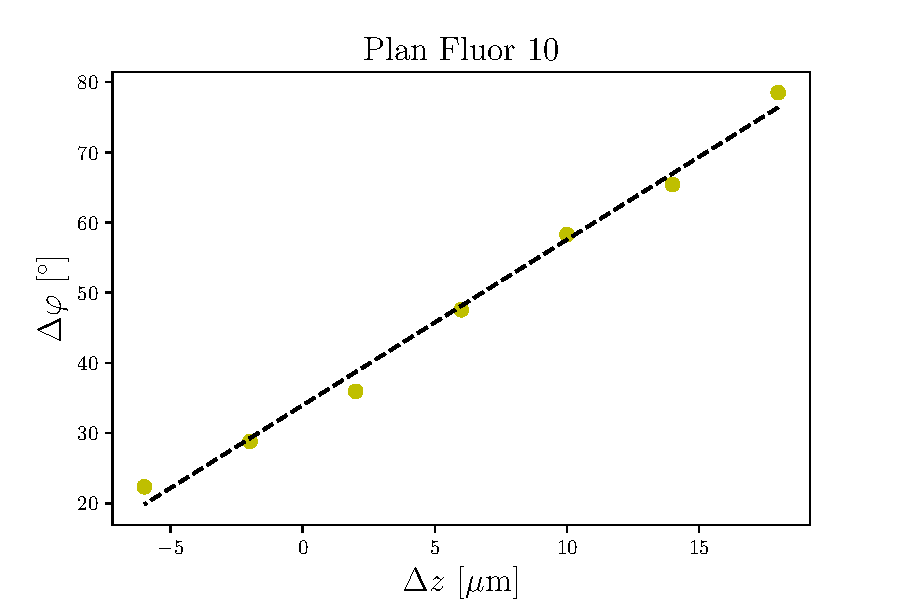
\includegraphics[width=\textwidth]{image/vysledek_10} 
			\caption{} %% aby se ti vysázelo označení obrázku.
		\end{subfigure}
		\begin{subfigure}[h]{0.63\textwidth}
			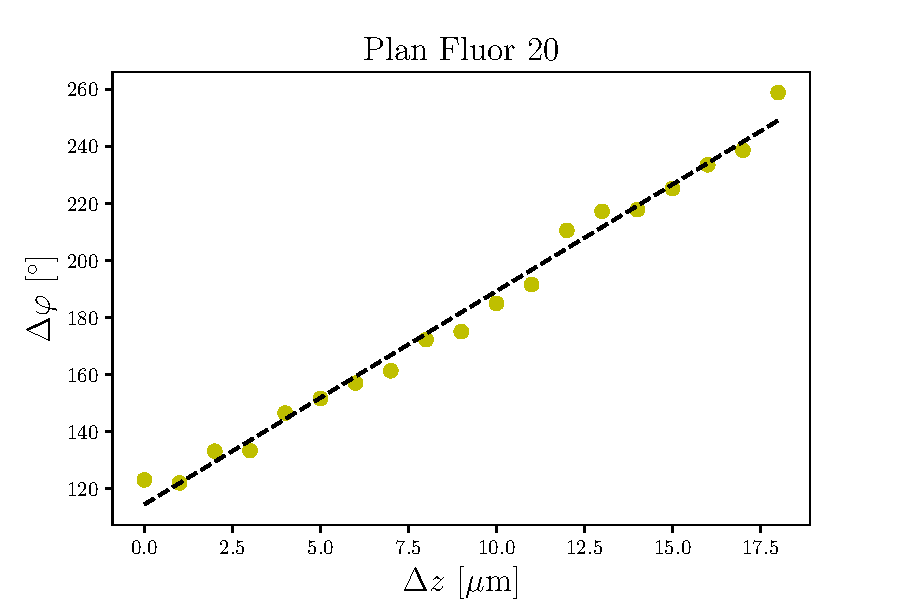
\includegraphics[width=\textwidth]{image/vysledek_20}
			\caption{}
		\end{subfigure}
		\caption[Graf závislosti rotace DH PSF $\Delta\varphi$ na defokusaci objektivu $\Delta z$.]{Graf závislosti rotace DH PSF $\Delta\varphi$ na defokusaci objektivu $\Delta z$, (a) při použití objektivu Plan Fluor 10, (b) při použití objektivu Plan Fluor 20. Měřená data (žluté body) jsou lineárně proloženy (přerušovaná přímka). }
		\label{fig:rotace_grafy}
	\end{figure}
	
		Pokud bys měl více podobrázků přichází do hry balíček \texttt{subcaption}. Pomocí něj lze vysázet i podobrázky. U podobrázků se popisek píše pouze jeden, dolů. Je v tomto připadě vhodné použít navíc hranaté závorky, do nichž se napíše kratší popisek, který se následně ukáže v seznamu obrázků.
	
	Všimni si, že obrázky jsou naschvál široké. Je to proto, aby byly dobře čitelné. Také si všimni popisku grafů. Ačkoli nejspíš netušíš co je to DH PSF či defokusace objektivu mělo by ti být jasné, že je důležité přesně graf popsat. To znamená co je na vodorovné ose, co je na svislé ose. V jakých jednotkách veličiny jsou. Které body co znamenají, která křivka má jaký význam. Napsat samotné \uv{$\Delta \varphi$} je málo, vždy raději připoměň, co daná značka znamená.
	

	
	\subsection{Literatura}
	
	V \LaTeX{}u lze dělat seznam literatury dvěma způsoby. V této šabloně jsem použil ten, kdy se seznam literatury píše přímo do práce. Pro jeho vygenerování doporučuji použít některý z generátarů, jako jsou například Citace PRO \cite{citacePRO}. Pomocí citací lze vygenerovat přímo dokument, který se pak už jen překopíruje do textu a člověk nemusí nic zvýrazňovat. Dále lze využít Bibtex, který rozhodně do budoucna hodlám zaimplementovat do šablony, avšak jeho použití nemusí být tak přátelské k začátečníkům.
	
	Pokud bys chtěl odkazovat na vícero zdrojů stačí je napsat vedle sebe oddělené čárkou \cite{LaTeXprirucka, citacePRO, Born2019}. Případně můžu odkaz na konkrétní stránku dát do hranatých závorek, viz \cite[str.~1]{Born2019}
	
	\subsection{Programový kód}
	Pro vložení programového kódu do dokumentu LaTeX s možností zvýraznění syntaxe můžete použít balíček \texttt{listings}. Tento balíček nabízí široké možnosti pro formátování kódu, včetně zvýraznění syntaxe pro různé programovací jazyky.
	
	Nejprve je třeba do preambule LaTeX dokumentu přidat \texttt{\\usepackage{listings}} a nastavit příslušné parametry. Příklad nastavení pro jazyk Python by mohl vypadat takto:
	

\begin{lstlisting}[style=Python, caption={Ukázka Python kódu}]
	# Python code here
	def hello_world():
		print("Hello, world!")
\end{lstlisting}


\begin{lstlisting}[style=JavaScript, title={Kód}, caption={Ukázka JS kódu}]
	// JavaScript code here
	function helloWorld() {
		console.log("Hello, world!");
	}
\end{lstlisting}	
	
\begin{lstlisting}[style=ES6, caption={ES6 (ECMAScript-2015) Listing}]
	/* eslint-env es6 */
	/* eslint-disable no-unused-vars */
	
	import Axios from 'axios'
	import { BASE_URL } from './utils/api'
	import { getAPIToken } from './utils/helpers'
	
	export default class User {
		constructor () {
			this.id = null
			this.username = null
			this.email = ''
			this.isActive = false
			this.lastLogin = ''  // ISO 8601 formatted timestamp.
			this.lastPWChange = ''  // ISO 8601 formatted timestamp.
		}
	}
	
	const getUserProfile = async (id) => {
		let user = new User()
		await Axios.get(
		`${BASE_URL}/users/${id}`,
		{
			headers: {
				'Authorization': `Token ${getAPIToken()}`,
			}
		}
		).then{response => {
				// ...
			}).catch(error => {
				// ...
			})
		}
\end{lstlisting}	
	
	\section[Pokročilejší tipy]{Pokročilejší tipy, které se mohou hodit}
	
	\subsection{Rovnice}
	
	Sazba matematiky je věda sama o sobě. Ačkoli Word prošel obrovskou změnou a je v~tomto mnohem lepší, tak \LaTeX je pro to přímo (ještě jsem neviděl matematika, co by používal Word). Spolu s balíčky \texttt{amsmath} a \texttt{amsfonts} snad neexistuje nic, co by se používalo a \LaTeX by to nezvládl. Ať už jde o základní věci jako řecká písmenka -- $\alpha, \beta, \gamma, \dots$ -- integrály -- $\int_{l_i}^{l_f} \tau \dif l $ -- až třeba po speciální písmena -- $\mathscr{F}: \mathbb{R}^n \to \mathbb{R}^m$. Pro případ, že bys potřeboval nějaké speciální integrály, je tu balíček \texttt{esint}, pomocí něj můžeš napsat třeba
	$$ \oiint_{S(V)} \vec{E} \cdot \dif \vec{S} = \iiint_{V} \left(\vec{\nabla} \cdot \vec{E}\right) \dif V .$$
	
	Jak můžeš vidět tak rovnice lze psát jednak do textu a nebo pokud se jedná o nějakou důležitou nebo rozsáhlejší rovnici tak na samostatný řádek. Pokud je rovnice opravdu důležitá, tak je vhodné ji také číslovat. Pak se na ni můžeš dále odkazovat v textu.
	\begin{equation}
		\vec{F} = m \vec{a}
		\label{eq:newton2}
	\end{equation}
	\dots Například podle druhého Newtonova zákona, rovnice (\ref{eq:newton2}) \dots Zároveň je vždy nutné vysvětlit co která veličina znamená. V tomto případě bych napsal, že v druhém Newtonově zákoně vektor síly $\vec F$ odpovídá součinu hmotnosti tělesa $m$ a jeho zrychlení $\vec a$. 
	
	Věřím, že se sazbou matematiky ti pomůže tvůj školitel, případně mi můžeš napsat (mail je v úvodu). Jednotlivé funkcionality spolu se seznamem znaků nalezneš jednak v Ne příliš stručném úvodu~\cite{LaTeXprirucka} nebo na Wikibooks v sekcích \emph{Mathematics} a \emph{Advanced mathematics}~\cite{wikibooksLaTeX}.
	
	
	
	
	\chapter{Když dokončuji práci}
	
	Každou práci je dobré zkontrolovat, aby v ní nebyly pravopisné chyby, nebyla těžkopádně napsaná -- byla čtivá -- a neobsahovala žádný typografický nedostatek. Proto, když práci sepíšeš, nech ji chvilku odležet, třeba týden. Pak si ji po sobě znovu přečti. Hned uvidíš, kolik věcí bys napsal jinak případně kde tě bije do očí jaká chyba. Dej práci přečíst také svému školiteli a případně češtináři. Zajistíš tak, že bude obsahovat méně chyb.
	
	Pak můžeš práci vytisknout a hurá do soutěže.
	
	\chapter*{Závěr}
	
	Věřím, že jsem ti spolu se šablonou poskytl několik tipů, jak napsat práci. Ať už jde o úplné začátky s \LaTeX{}em. Či ukázku toho, co vše s ním zvládneš. Pokud bys měl k šabloně libovolné dotazy, rouhodně se na mě obrať. \LaTeX tvé práci dodá určitou krásu, tak doufám, že ti dodá sebevědomí a uspěješ při souteži. A i kdyby ne vzpomeň si, kolik ses toho musel naučit a hned uvidíš o jaký kus ses posunul.
	
	%% literatura
	\begin{thebibliography}{99}
		\bibitem{sablonaSOC} DOKULIL Jakub. \textit{Šablona pro psaní SOČ v programu \LaTeX} [Online]. Brno, 2020 [cit. 2020-08-24]. Dostupné z: \url{https://github.com/Kubiczek36/SOC_sablona}
		\bibitem{LaTeXprirucka}OETIKER, Tobias, Hubert PARTL, Irene HYNA, Elisabeth SCHEGL, Michal KOČER a Pavel SÝKORA. \textit{Ne příliš stručný úvod do systému LaTeX2e} [online]. 1998 [cit. 2020-08-24]. Dostupné z: \url{https://www.jaroska.cz/elearning/informatika/typografie/lshort2e-cz.pdf}
		\bibitem{wikibooksLaTeX}\textit{Wikibooks: LaTeX} [online]. San Francisco (CA): Wikimedia Foundation, 2001- [cit. 2020-08-24]. Dostupné z: \url{https://en.wikibooks.org/wiki/LaTeX}
		\bibitem{stackExchange} \textit{TeX - LaTeX Stack Exchange} [online]. Stack Exchange, 2020 [cit. 2020-09-01]. Dostupné z: \url{https://tex.stackexchange.com}
		\bibitem{sspuLogo} \textit{Střední škola průmyslová a umělecká Opava} [online]. [cit. 2023-11-11]. Dostupné z: \url{https://www.sspu-opava.cz}
		\bibitem{citacePRO}\textit{Citace PRO} [online]. Citace.com, 2020 [cit. 2020-08-31]. Dostupné z: \url{https://www.citacepro.com}
		\bibitem{Born2019} BORN, Max a Emil WOLF. \textit{Principles of optics: electromagnetic theory of propagation, interference and diffraction of light}. 7th (expanded) edition. Reprinted wirth corrections 2002. 15th printing 2019. Cambridge: Cambridge University Press, 2019. ISBN 978-0-521-64222-4.
	\end{thebibliography}
	
	%% obrázky 
	\listoffigures
	
	%% tabulky
	\listoftables
	
	\appendix %% začínají přílohy
	
	\titleformat{\chapter}[block]{\scshape\bfseries\LARGE}{Příloha \thechapter}{10pt}{\vspace{0pt}}[\vspace{-22pt}] %% nastavení nadpisu u příloh
	
	
	\chapter{%Příloha A 
		Spot diagramy a další }
	
	
\end{document}